\chapter[Referencial Teórico]{Referencial Teórico}
Este Capítulo apresenta as bases teóricas que suportam esse trabalho. Estando organizado em seções, sendo estas:
Seção \hyperref[sec:sisrec]{2.1}, que apresenta Sistemas de Recomendação; Seção \hyperref[sec:ia]{2.2}, a qual traz 
o conceito de Inteligência Artificial e recursos desta que serão utilizados neste trabalho; Seção \hyperref[sec:expus]{2.3},
que aborda a experiência do usuário e sua importância para este trabalho. E por último, são apresentadas as considerações finais
do capítulo.

\section{Sistemas de Recomendação}\label{sec:sisrec}

Os Sistemas de Recomendação são aplicações de software que analisa e processa dados dos usuários com o proposito de 
sugerir itens que possam ser de interesse desses usuários. Assim, eles ajudam os usuários a descobrir novos produtos, 
conteúdos ou serviços que possam ser do seu interesse, personalizando suas experiências \cite{pham2019recommendation}.

\begin{figure}[h]
    \centering
    \includegraphics[width=0.5\textwidth]{figuras/ciclosr.eps}
    \caption{Ciclo dos Sistemas Recomendação}
    \label{fig:ciclosr}
    \small Fonte: Autora
\end{figure}

O processo de um sistema de recomendação pode ser dividido em várias etapas, como demonstrado na figura 
\hyperref[fig:ciclosr]{1}. O ciclo começa na coleta de dados, nesta etapa o sistema coleta dados relevantes para analise
do perfil do usuário, como interações com o sistema, \textit{feedbacks}, fontes externas como midias sociais também podem ser
dados válidos. Como o (Kurt and Murali, 2016) exemplificam, o Spotify coleta informações dos artistas, sinais acústicos das músicas,
histórico e em tempo real músicas ouvidas.
Após a coleta, temos o armazenamento e filtragem desses dados, em geral para popular a base de dados, quanto maior a quantidade de dados,
melhor para a análise e separar esses dados para melhorar a acurácia do modelo \cite{pham2019recommendation}. Em seguida, 
temos a análise desses dados, no caso desse trabalho, utilizando algoritmos de \textit{deep learning} para detectar padrões,
e encontrar as preferências do usuário. Dessa forma, conseguindo gerar recomendações em potencial que serão sugeriadas para o usuário,
entrando na última parte do ciclo, que é a avaliação pelo usuário da recomendação, e com base nessa avaliação, o modelo 
de recomendação recebe mais dados do perfil daquele usuário e o ciclo recomeça.

\section{Inteligência Artificial}\label{sec:ia}

Inteligência Artificial é um conjunto de tecnologias que permitem aos computadores executar uma variedade de 
funções avançadas, incluindo a capacidade de ver, entender e traduzir idiomas falados e escritos, analisar dados, 
fazer recomendações e muito mais \cite{Suleimenov}.

No contexto de Sistemas de Recomendação, é feito o uso principalmente de quatro técnicas da Inteligência Artificial 
\cite{stratoflow-recommendation}:
\begin{itemize}
\item Filtros colaborativos: essa técnica foca na similaridade entre diferentes usuários e itens. Usuários que são
similares provavelemente tem o mesmo tipo de interesse \cite{pham2019recommendation}, como demonstrado na Figura 
\hyperref[fig:filtrocolab]{2};

\begin{figure}[htbp]
    \centering
    \includegraphics[width=0.5\textwidth]{figuras/filtrocolab.eps}
    \caption{Filtro Colaborativo}
    \label{fig:filtrocolab}
    \small Fonte: Autora
\end{figure}

\item Filtros de conteúdo: essa técnica avalia a similaridade entre os itens, itens similares ao que o usuário gostou/visualizou
tem mais probabilidade de ser de seu interesse \cite{stratoflow-recommendation}, demonstrado na Figura 
\hyperref[fig:filtrocont]{3};

\begin{figure}[htbp]
    \centering
    \includegraphics[width=0.5\textwidth]{figuras/filtrocontent.eps}
    \caption{Filtro de Conteúdo}
    \label{fig:filtrocont}
    \small Fonte: Autora
\end{figure}

\item Filtros demográficos: essa técnica busca categorizar os usuários com base em atributos e fazer recomendações
com base em classes \cite{burke2002hybrid}. 

\item Filtros baseado em conhecimento e utilidade: essa técnica recomenda com base nas necessidades dos usuários, 
calculando a utilidade de cada item para o usuário, para isso é necessário conhecimento do que o usuário precisa e 
quais os itens que suprem essa necessidade \cite{burke2002hybrid}.Como por exemplo, um usuário pesquisa por um restaurante
italiano específico (como Peccorino), o sistema de recomendação buscaria quais são os itens que tem maior utilidade para 
o usuário, nesse caso sugerindo outro restaurante italiano similar.

\item Filtros Híbridos: essa técnica combina outras técnicas de filtragem, como por exemplo Filtros colaborativos e Filtros
de conteúdo. Possui várias formas de combinar essas técnicas, que serão abordadas na seção 
\hyperref[subsubsec:tiposfh]{Classificação de Filtros Híbridos}. Esta técnica consegue lidar com as limitações das técnicas que 
ela combina, podend, por exemplo, lidar com usuários de gostos mais diferentes e com situações as quais
tem poucos dados de interação do usuário, assim também lidando com o problema de 
"partida à frio"\cite{stratoflow-recommendation}, e 

\item Filtros baseados em \textit{Deep Learning}: essa técnica utiliza redes neurais para fazer predições e recomendações, 
como Redes Neurais Convolucionais (RNC), para dados mais voltados para imagens, e Redes Neurais Recorrentes (RNR), para dados
sequênciais \cite{nvidia-recommendation}.
\end{itemize}

Para esse trabalho, será abordado mais afundo os seguintes filtros:
\hyperref[subsec:hibridos]{Filtros Híbridos} e \hyperref[subsec:filtrodeep]{Filtros baseados em \textit{Deep Learning}}.

\subsection{Filtros Híbridos}\label{subsec:hibridos}
A filtragem hibrida aborda mais de um tipo de técnica de filtragem, visando superar os lados negativos que essas filtragens
tem ao estarem separadas, problemas como \textit{cold start} e diversidade e esparcidade dos dados. Esse modelo, também surgiu
na tentativa de melhorar a acurácia do processo de recomendação \cite{thorat2015survey}.

\subsubsection{Classificação de Filtros Híbridos}\label{subsubsec:tiposfh}
De acordo com Robin Burke (2002) os modelos com filtragem hibrida voltados para Sistemas de Recomendação podem possuir
várias classificações, baseado em como combinam os outros tipos de filtro. Alguns dessas classificações são:

\begin{itemize}
    \item Por peso (\textit{Weighted}): Apresenta um sistema de peso, que o peso de um item é calculado com base no resultado
    de sua avaliação por todas as técnicas presentes no sistema. Esse tipo tem como base que todas as técnicas produziriam
    valores relativos similares, mas esse nem sempre é o caso, assim alguns itens com poucas classificações podem ser ignorados;

    \item Por troca (\textit{Switching}): O sistema troca entre diferentes técnicas de recomendação dependendo do contexto.
    Esse tipo adiciona uma complexidade a mais ao sistema, já que precisa definir o critério para troca entre as técnicas,
    mas também permite aproveitar os benefícios de várias técnicas;

    \item Por mistura (\textit{Mixed}): Apresenta recomendações de mais de uma técnica juntas. Esse modo reduz parcialmente
    o problema de "patida à frio", para novos itens é possível classificá-los com base na sua descrição, porém para novos
    usuários o problema de não ter informações suficiente permanece; 

    \item Por combinação de \textit{features} (\textit{Feature Combination}): Usa os dados do filtro colaborativo como dados
    adicionais associados a cada exemplo e usar filtros de conteúdos na base aumentada que será gerada. Esse tipo considera
    os dados gerados pelos filtros colaborativos, sem necessariamente depender deles, assim reduz o problema da falta de dados
    \textit{cold start};

    \item Por cascata (\textit{Cascade}): Usa uma técnica para produzir uma classificação grosseira dos dados e em seguida
    usa outra técnica para refinar essa classificação. Esse tipo evita que itens sejam ignorados, como pode ocorrer na técnica
    de peso que aplica a técnica a todos os itens, pois no cascata as classificações são apenas refinadas e não substituidas; 

    \item Por aumento de \textit{features} (\textit{Feature Augmentation}): Usa um modelo gerado por uma técnica de filtro
    para produzir uma classificação ou avaliação de um item e essa informação produzida vai ser introduzida em outro 
    modelo, gerado por outra técnica de filtro, a ser utilizado. Esse tipo de
    sistema hibrído pode aumentar a performance do sistema sem modificá-lo diretamente, e

    \item Por \textit{Meta-level} (\textit{Meta-level}): Usa um dos modelos gerados pelas técnicas como entrada 
    para o outro modelo a ser gerado por outra técnica.
    Como por exemplo, usar o modelo gerado por filtros colaborativos como entrada para um modelo por filtro de conteúdo.
    Nesse caso em específico, o \textit{Meta-level} tem o benefício de que o modelo final vai ser uma representação fiel
    dos interesses do usuário e facilita a operação do sistema ao usar essa representação ao se comparar com dados crus 
    de avaliação.
\end{itemize}

A Figura \hyperref[fig:allhybrid]{4} apresenta uma tabela com as possíveis combinações de filtros para formar um filtro
hibrído, bem como atuais sistemas que usam essas combinações.
\begin{figure}[htbp]
    \centering
    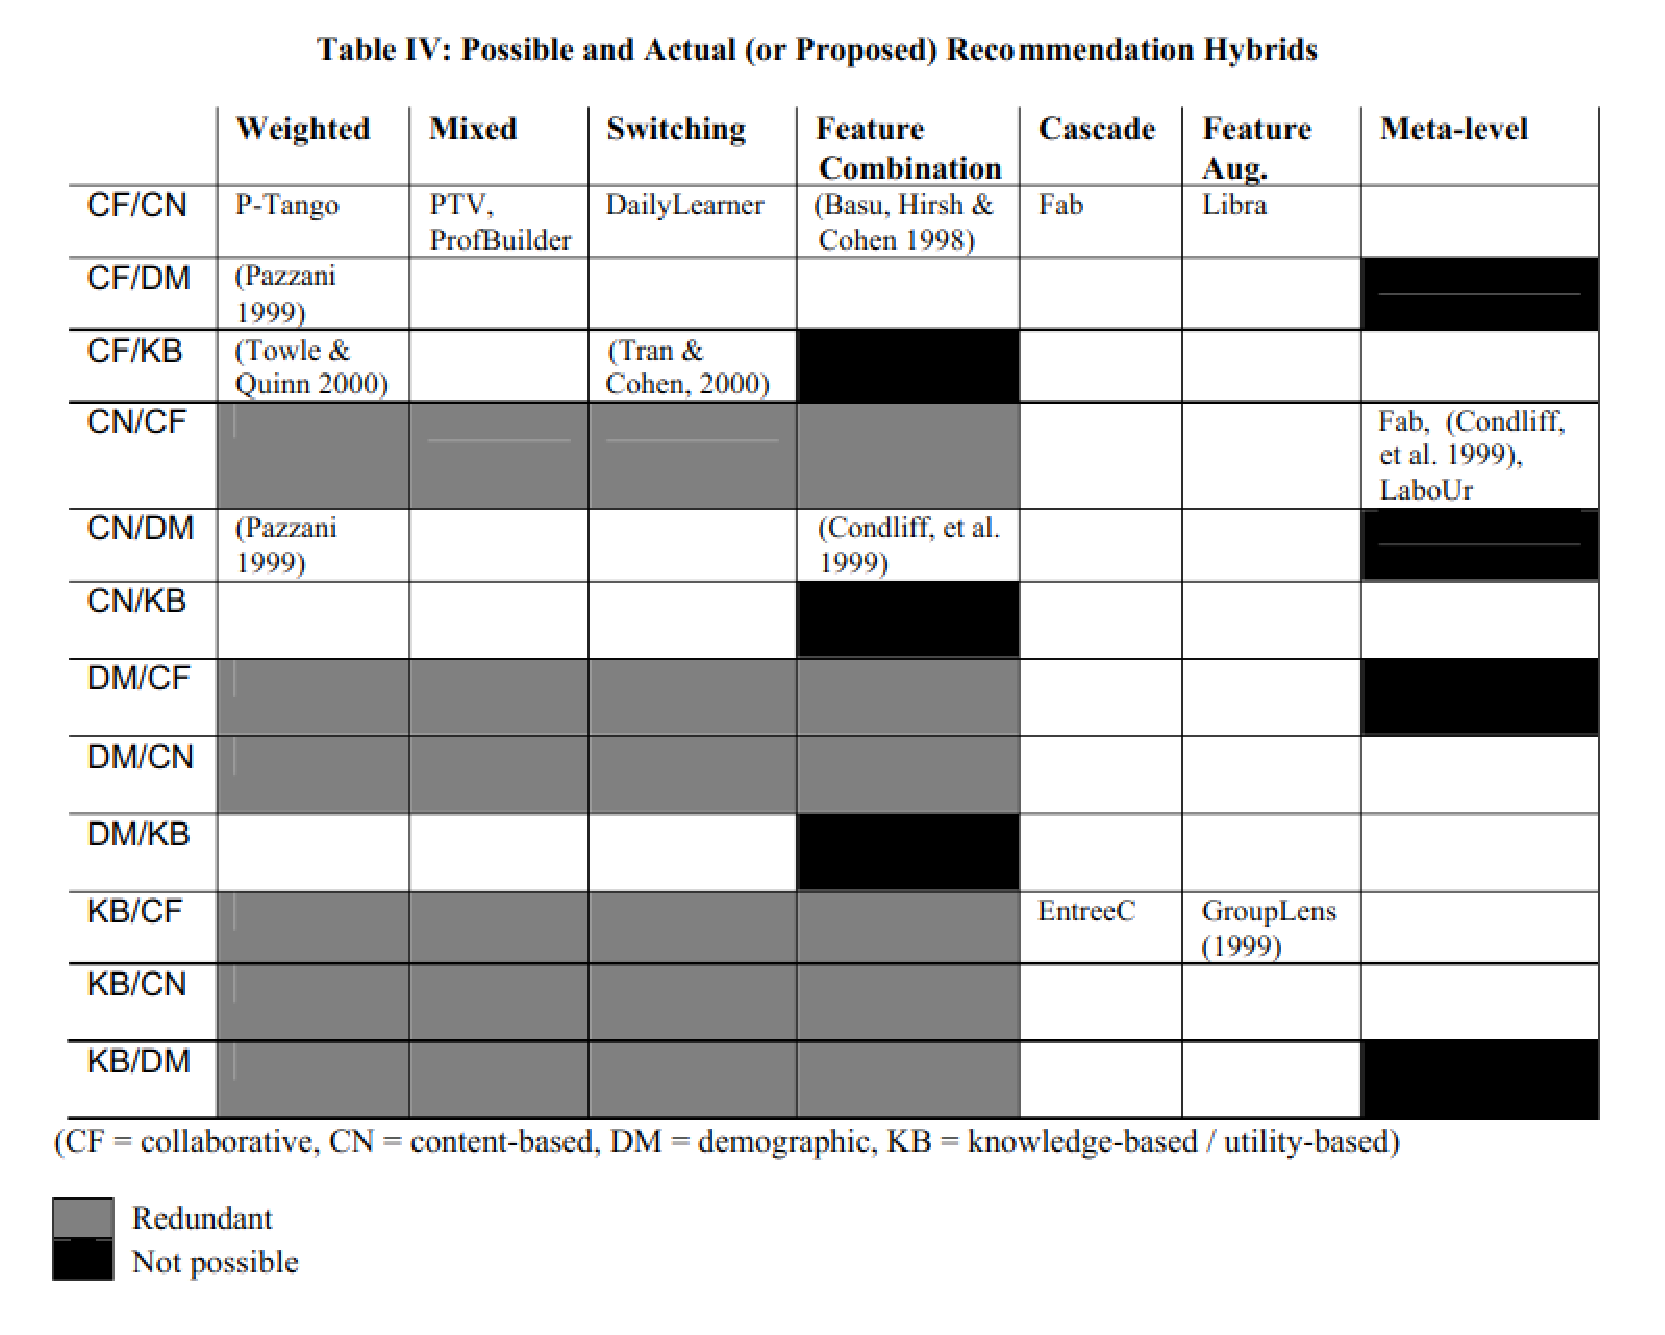
\includegraphics[width=0.5\textwidth]{figuras/allhybrid.eps}
    \caption{Sistemas de Recomendação com Filtro Híbrido}
    \label{fig:allhybrid}
    \small Fonte: \cite{burke2002hybrid}
\end{figure}

\subsubsection{Possíveis implementações}\label{subsubsec:implemfh}
No contexto desse trabalho, o filtro híbrido a ser discutido será uma combinação de filtros colaborativos e filtros de 
conteúdo. No quesito de implementação da combinação desses filtros, fortemente baseadas nas classificações dos filtros 
híbridos, temos as possibilidades como exemplificado por THORAT; GOUDAR; BARVE (2015):

\begin{itemize}
    \item Implementar os filtros separadamente e juntá-los para realizar a recomendação, como exemplificado na figura
    \hyperref[fig:combind]{5};
    \begin{figure}[htbp]
        \centering
        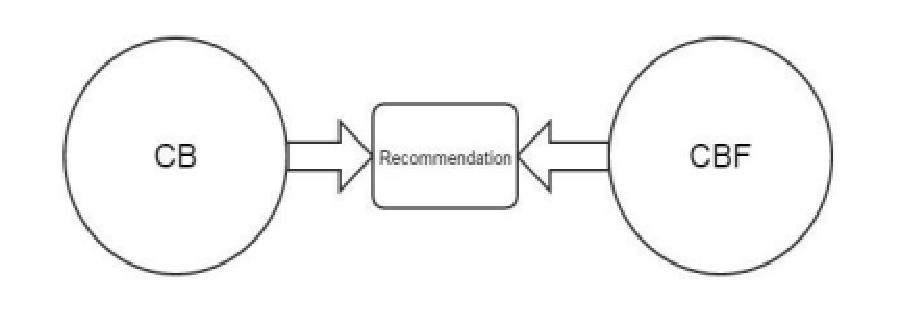
\includegraphics[width=0.5\textwidth]{figuras/combind.eps}
        \caption{Combinação individual}
        \label{fig:combind}
        \small Fonte: \cite{thorat2015survey}
    \end{figure}

    \item Implementar características do filtro de conteúdo no filtro colaborativo, como exemplificado na figura
    \hyperref[fig:cfcbf]{6};
    \begin{figure}[htbp]
        \centering
        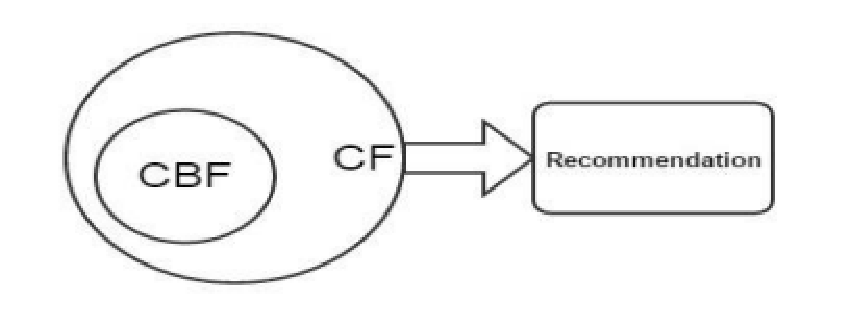
\includegraphics[width=0.5\textwidth]{figuras/cfcbf.eps}
        \caption{Agregar conteúdo dentro de colaborativo}
        \label{fig:cfcbf}
        \small Fonte: \cite{thorat2015survey}
    \end{figure}

    \item Unificar os filtros em um único modelo, como exemplificado na figura
    \hyperref[fig:modelounico]{7}, e
    \begin{figure}[htbp]
        \centering
        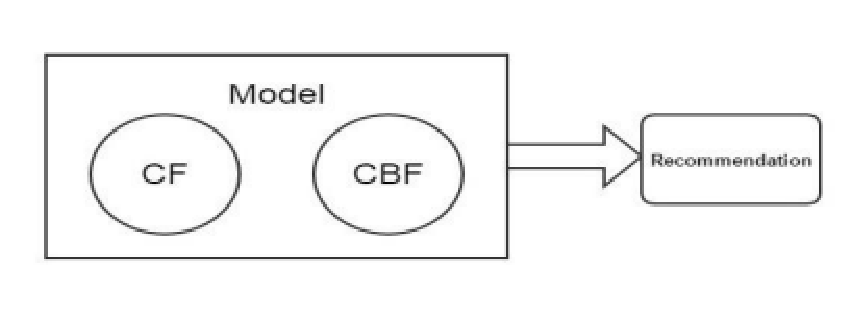
\includegraphics[width=0.5\textwidth]{figuras/modelounico.eps}
        \caption{Ambos os filtros em um único modelo}
        \label{fig:modelounico}
        \small Fonte: \cite{thorat2015survey}
    \end{figure}

    \item Implementar características do filtro colaborativo no filtro de conteúdo, como exemplificado na figura
    \hyperref[fig:cbfcf]{8}.
    \begin{figure}[htbp]
        \centering
        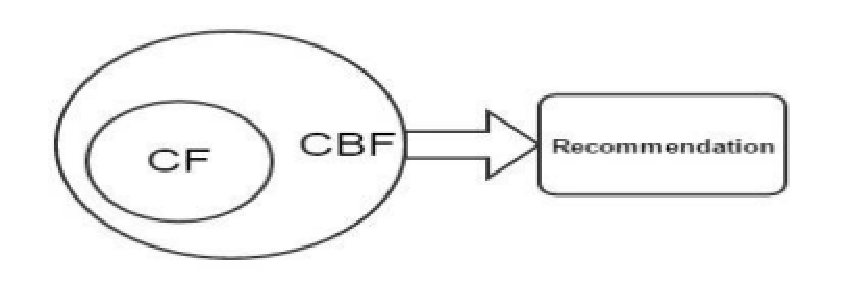
\includegraphics[width=0.5\textwidth]{figuras/cbfcf.eps}
        \caption{Agregar colaborativo dentro de conteúdo}
        \label{fig:cbfcf}
        \small Fonte: \cite{thorat2015survey}
    \end{figure}
\end{itemize}

\subsection{Filtros baseados em \textit{Deep Learning}}\label{subsec:filtrodeep}
\textit{Deep Learning} é uma sub-área de Inteligência Artificial que se concentra no treinamento de algoritmos para 
realização de tarefas complexas de forma autônoma, e permite que esses algoritmos aprendam representações de 
dados com múltiplas camadas de abstração \cite{LeCun2015}. Focando em Sistemas de Recomendação, 
podemos melhorar os outros filtros existentes ao usar \textit{Deep Learning}. Nesse sentido, temos quatro possíveis 
abordagens: Redes Neurais Convolucionais; Redes Neurais Recorrentes; Máquina de Boltzmann restrita e Autoencoder 
\cite{elSisi2020}.

\subsubsection{Redes Neurais Convolucionais}\label{subsubsec:rnc}
É um tipo de rede neural com camadas convolucionais e operações de agrupamento \cite{elSisi2020}.

No escopo de Sistemas de Recomendação, são ideais para processar dados de multimídia, conseguindo associat dados de 
diferentes formatos, assim melhorando a precisão das recomendações.

\subsubsection{Redes Neurais Recorrentes}\label{subsubsec:rnr}
É um tipo de rede neural que possui \textit{loops} e guarda cálculos anteriores, ideal para modelar data sequencial 
\cite{elSisi2020}.

Aplicando esse método em Sistemas de Recomendação, consegue identificar padrões no comportamento e interações dos usuários,
consegue criar recomendações baseadas na navegação do usuário na rede, sem precisar de dados iniciais informados pelos
usuários, como o que ocorre na geração de \textit{cookies} \cite{elSisi2020}. Dessa forma, consegue lidar com o problema 
da "partida à frio".

\subsubsection{Máquina de Boltzmann restrita}\label{subsubsec:boltzmann}
A Máquina de Boltzmann restrita é uma rede neural de dupla camada, uma visível e outra escondida \cite{elSisi2020}. 

Para Sistemas de Recomendação, pode ser interligada com filtros colaborativos para aumentar o tamanho da base de dados,
assim melhorando o processo de recomendação \cite{elSisi2020}. Ela também pode ser treinada para aprender uma representação
dos padrões de interação entre usuários e itens, para posteriormente gerar recomendações com base nas preferências dos
usuários e nas características dos itens.

\subsubsection{\textit{Autoencoder}}\label{subsubsec:autoencoder}
\textit{Autoencoder} é uma rede neural que tenta reconstruir seu dado de entrada em um dado similar na saída, ao usar uma
camada mediadora \cite{elSisi2020}. Possuindo, assim, três camadas, as quais o número de neurônios na entrada deve ser igual ao número de
neurônios na saída, como exemplificado na figura \hyperref[fig:autoencoder]{9}.
\begin{figure}[htbp]
    \centering
    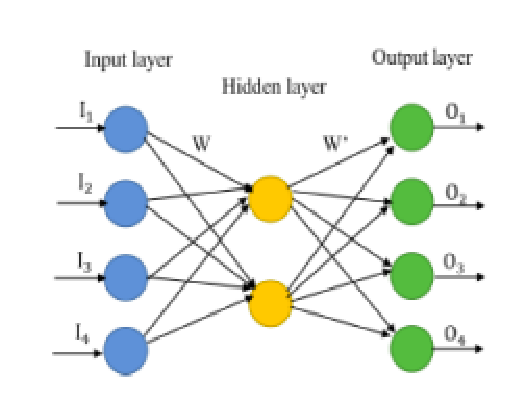
\includegraphics[width=0.5\textwidth]{figuras/autoencoder.eps}
    \caption{Estrutura de um \textit{Autoencoder}}
    \label{fig:autoencoder}
    \small Fonte: \cite{elSisi2020}
\end{figure}

No contexto de Sistemas de Recomendação, tem a habilidade de reduzir e reconstruir os dados e extrair os atributos destes.
E por isso um \textit{Autoencoder} pode ser treinado para aprender representações latentes dos itens, as quais capturam as características
essenciais dos itens e podem ser usadas para recomendar itens semelhantes com base em similaridade. Eles também podem
ser usados para aprender representações dos usuários e itens a partir de interações históricas de usuários com itens e fazer
recomendações com base em padrões de comportamento. E por fim, eles podem ainda aprender diferentes tipos de informações com
base em diferentes tipos de dados de entrada (áudio, imagem, texto) e combinar essas modalidades para gerar a recomendação \cite{zhang2020autoencoder}.

% \subsection{Modelo a ser usado}\label{subsec:modeloaserusado}

\section{Experiência do usuário}\label{sec:expus}
A experiência do usuário pode ser definida como as respostas e percepções de uma pessoa ao usar um produto, sistema ou serviço
\cite{iso9241-210}. Mas também podemos dizer que a experiência de usuário vai além de avaliar a usabilidade/funcionalidade durante
a interação do usuário, ela tende a cobrir não só os comportamentos do sistema, bem como a eficiência e efetividade \cite{allam2013user}
No contexto de Sistemas de Recomendação, a experiência do usuário como apontado por \cite{8673410} aumenta a precisão e eficiência
das recomendações. Por isso, esse trabalho tem o intuito de levantar considerações dos usuários acerca do sistema e usar esses
dados para o aprendizado da Inteligência Articial por trás do Sistema de Recomendação. 

\section{Resumo do Capítulo}\label{sec:resrefteor}

Esse capítulo apresentou uma ideia geral do que são Sistemas de Recomendação, um sistema que visa recomendar coisas que 
sejam do interesse dos usuários, bem como suas etapas (coleta, armazenamento, filtro, analise, geração de dados e 
avaliação das recomendações). Também foi mostrado os diversos filtros para Sistemas de Recomendação usando Inteligência 
Articial, sendo eles colaborativo, por conteúdo, demográfico, baseado em conhecimento e utilidade, híbridos e baseados em
\textit{Deep Learning}.

Com o foco em filtros híbridos e filtros baseados em deep learning, foi detalhado mais como eles funcionam e suas definições.
Para os filtros híbridos, que são combinações de outros filtros (colaborativo e por conteúdo, no contexto deste trabalho),
foi apresentado sua classificação: por peso, que pondera os resultados dos filtros que são combinados; por mistura, que 
apresenta em conjunto o resultados dos outros filtros; por troca, que alterna entre os filtros com base em um critério;
por combinação de \textit{features} que usa dados de um dos filtros para aumentar a base de dados do outro filtro a ser usado;
por cascata, que usa um filtro para produzir uma classificação e outro filtro para refinar essa classificação; por aumento
de \textit{features}, que o resultado de um filtro é a entrada de outro filtro; e por último por \textit{Meta-level}, que
o modelo gerado por um filtro é usado de entrada em outro filtro.

Para os filtros baseados em textit{Deep Learning}, foi visto que temos quatro possíveis metódos, sendo eles: Redes Neurais 
Convolucionais, que auxília na interpretação e associação de diferentes formatos de dados; Redes Neurais Recorrentes, 
que consegue aprender padrões de uso do usuário; Máquina de Boltzmann restrita, que pode gerar representações de usuários
e itens para melhorar o processo de recomendação; e por fim Autoencoder, que pode tanto combinar diferentes multimídias quanto 
gerar representações de usuários para melhorar as recomendações.

E ainda, esse capítulo traz a importância da experiência de usuário em Sistemas de Recomendação, e como isso será abordado
no trabalho.